%!TEX TS-program = xelatex
%!TEX root = ../Topo2_WS15/topologie_2.tex
\RequirePackage{fix-cm} 
\documentclass[a4paper, twoside, headsepline, index=totoc,toc=listof, fontsize=10pt, cleardoublepage=empty, headinclude, DIV=12, BCOR=5mm, titlepage,draft]{scrartcl}
\usepackage{scrtime} % KOMA, Uhrzeit ermoeglicht

\usepackage{etoolbox}
\usepackage{letltxmacro}
\usepackage{ifthen}

%--Farbdefinitionen
%-- muss vor tikz geladen werden
\usepackage[usenames, table, x11names]{xcolor}
\definecolor{dark_gray}{gray}{0.45}
\definecolor{light_gray}{gray}{0.6}
\usepackage[final]{graphicx}

%--Zum Zeichnen
%-- muss vor polyglossia bzw. babel geladen werden
\usepackage{tikz}
\usepackage{tikz-cd}
\usetikzlibrary{external}
\tikzset{>=latex}
\usetikzlibrary{shapes,arrows.meta,intersections}
\usetikzlibrary{calc,3d}
\usetikzlibrary{decorations.pathreplacing,decorations.markings, decorations.pathmorphing}
\usetikzlibrary{angles}

%-- Konfiguration von tikzexternalize
\tikzexternalize[prefix=tikz/,up to date check=diff]
\pgfkeys{/pgf/images/include external/.code=\includegraphics{#1}}
\tikzset{external/system call={xelatex \tikzexternalcheckshellescape -halt-on-error -interaction=batchmode --shell-escape -jobname "\image" "\texsource"}}


%-- tikzexternalize fuer tikzcd deaktivieren, da inkompatibel
\AtBeginEnvironment{tikzcd}{\tikzexternaldisable}
\AtEndEnvironment{tikzcd}{\tikzexternalenable}

%-- um Inkompatibilitaeten von quotes und polyglossia bzw. babel zu vermeiden
\tikzset{
  every picture/.append style={
    execute at begin picture={\shorthandoff{"}},
    execute at end picture={\shorthandon{"}}
  }
}
\usetikzlibrary{quotes}
\usepackage{pgfplots}
\usepgfplotslibrary{colormaps}
% \pgfplotsset{compat=1.12}



%-- Mathesymbole etc.
\usepackage{mathtools} % beinhaltet amsmath
\mathtoolsset{showonlyrefs, centercolon,showmanualtags}
\newtagform{brackets}[\textbf]{[}{]}
\usetagform{brackets}
\usepackage{fix-cm}
% \usepackage{wasysym} % zusätzliche Symbole
\usepackage{amssymb} % zusätzliche Symbole
% \usepackage{stmaryrd} % für Blitz
\usepackage{nicefrac} % schräge Brüche
\usepackage{faktor}
\newcommand{\Faktor}[1]{\faktor[\textstyle]{#1}}
\usepackage{xfrac}
\usepackage{cancel}
\usepackage{mathdots} % Verbesserung von Punkten wie zB \ldots
\usepackage[bb=px]{mathalfa}

%-- einzelne Symbole aus dem mathx-package
% \DeclareFontFamily{U}{mathx}{\hyphenchar\font45}
% \DeclareFontShape{U}{mathx}{m}{n}{<-> mathx10}{}
% \DeclareSymbolFont{mathx}{U}{mathx}{m}{n}
% \DeclareMathSymbol{\bigplus}{1}{mathx}{"90}

%-- 
\usepackage{silence}
\WarningFilter{latexfont}{Size substitutions with differences}
\WarningFilter{latexfont}{Font shape `U/bbold/m/n' in size}

\DeclareSymbolFont{bbold}{U}{bbold}{m}{n}
\DeclareSymbolFontAlphabet{\mathbbold}{bbold}
\newcommand{\ind}{\mathbbold{1}} % charakteristische-Funktion-Eins

\def\mathul#1#2{\color{#1}\underline{{\color{black}#2}}\color{black}} %farbiges Untersteichen im Mathe-Modus
\renewcommand{\le}{\leqslant}
\renewcommand{\ge}{\geqslant}

%-- Underbrace als Befehl in LaTeX-Syntax (und ohne Spacingprobleme mit nachfolgenden Operatoren...)
\newcommand{\Underbrace}[2]{{\underbrace{#1}_{#2}}}
\newcommand{\Underbracket}[2]{{\underbracket[0.7pt][2pt]{#1}_{#2}}}

%-- Alles was mit Schrift und XeTeX zu tun hat
\usepackage{palatino}
\usepackage[euler-digits]{eulervm}
\usepackage[no-math]{fontspec}
\usepackage{polyglossia} % moderner babel-ersatz
\setmainlanguage[spelling=new,babelshorthands=true]{german}
\shorthandoff{"}
\setotherlanguage{english}
\defaultfontfeatures{Mapping=tex-text, WordSpace={1.2}, Ligatures={Required,Common,Contextual}} %

%-- Alle hier aufgeführten Schriftarten sind in jeder TeXlive-Installation vorhanden!!
%-- Hauptschriftart festlegen
% \setmainfont{texgyrepagella}[Extension=.otf,UprightFont=*-regular,BoldFont=*-bold,ItalicFont=*-italic,BoldItalicFont=*-bolditalic,ItalicFeatures={Style=Historic}]
\setmainfont{TeXGyrePagellaX}[Extension=.otf,UprightFont=*-Regular,BoldFont=*-Bold,ItalicFont=*-Italic,BoldItalicFont=*-BoldItalic,ItalicFeatures={Style=Historic},Ligatures={Required,Common,Contextual,Historic}]
% \setmainfont[BoldFont={* Bold}, ItalicFont={* Light Italic},SmallCapsFont={Linux Libertine O}, SmallCapsFeatures={Letters=SmallCaps}]{Source Sans Pro}


%-- Serifenlose Schriftart festlegen
% \setsansfont{Roboto}[Scale=MatchUppercase,Extension=.ttf,UprightFont=*-Regular,BoldFont=*-Bold,ItalicFont=*-RegularItalic,BoldItalicFont=*-MediumItalic]
% \setsansfont{RobotoSlab}[Scale=MatchUppercase,Extension=.ttf,UprightFont=*-Regular,BoldFont=*-Bold,ItalicFont=*-Thin,SmallCapsFont=*-Regular]
% \setsansfont{FiraSans}[Scale=MatchUppercase,Extension=.otf, UprightFont=*-Regular, BoldFont=*-SemiBold, ItalicFont=*-RegularItalic, BoldItalicFont=*-MediumItalic]
% \setsansfont{SourceSansPro}[Scale=MatchUppercase,Extension=.otf,UprightFont=*-Regular,BoldFont=*-Semibold,ItalicFont=*-LightIt,BoldItalicFont=*-SemiboldIt]
% \setsansfont{texgyreadventor}[Scale=MatchUppercase, Extension=.otf, UprightFont=*-regular, BoldFont=*-bold, ItalicFont=*-italic,BoldItalicFont=*-bolditalic]
% \setsansfont{Kurier}[Scale=MatchUppercase, Extension=.otf, UprightFont=*Medium-Regular, BoldFont=*Heavy-Regular, ItalicFont=*Medium-Italic,BoldItalicFont=*Heavy-Italic]
% \setsansfont{Iwona}[Scale=MatchUppercase, Extension=.otf, UprightFont=*Medium-Regular, BoldFont=*Heavy-Regular, ItalicFont=*Medium-Italic,BoldItalicFont=*Heavy-Italic]
% \setsansfont{LinBiolinum}[Scale=MatchUppercase, Extension=.otf, UprightFont=*_R, BoldFont=*_RB, ItalicFont=*_RI,BoldItalicFont=*_RBO]
% \setsansfont{texgyrebonum}[Scale=MatchUppercase,Extension=.otf, UprightFont=*-regular, BoldFont=*-bold, ItalicFont=*-italic, BoldItalicFont=*-bolditalic]
\setsansfont{texgyreadventor}[Scale=MatchUppercase,Extension=.otf, UprightFont=*-regular, BoldFont=*-bold, ItalicFont=*-italic, BoldItalicFont=*-bolditalic]



% \newfontfamily{\geometric}{texgyreheros}[Scale=MatchLowercase, Extension=.otf, UprightFont=*-regular, BoldFont=*-bold, ItalicFont=*-italic]
% \addtokomafont{disposition}{\geometric}
\setmonofont{SourceCodePro}[Scale=0.9,Extension=.otf,UprightFont=*-Regular, BoldFont=*-Semibold, ItalicFont=*-Light]
\usepackage{xltxtra}
\usepackage{fontawesome}
\usepackage[final]{microtype}


\usepackage[draft=false]{scrlayer-scrpage} % wie fancyhdr, nur optimiert auf KOMA-Skript, leicht andere Syntax

\flushbottom


%--Mixed
\usepackage[shortlabels,inline]{enumitem}
\setlist[itemize,1]{label=\faCaretRight}
\setlist[enumerate]{font=\bfseries}
\setlist[description]{font=\normalfont\bfseries}
\usepackage[german=quotes]{csquotes}
\usepackage{makeidx}
\usepackage{wrapfig}
\usepackage{float}
\usepackage[margin=10pt, font=small, labelfont={sf, bf}, format=plain, indention=1em]{caption}
\captionsetup[wrapfigure]{name=Abb. }
\usepackage{stackrel}


%--Unterstreichung
\usepackage[normalem]{ulem}
\setlength{\ULdepth}{1.8pt}

%--Indexverarbeitung
\newcommand{\bet}[1]{\emph{#1}}
\newcommand{\Index}[1]{\bet{#1}\index{#1}}
\makeindex
\setindexpreamble{{\noindent\sffamily\small Die \emph{Seitenzahlen} sind mit Hyperlinks versehen und somit anklickbar}  \par \bigskip}
\renewcommand{\indexpagestyle}{scrheadings}


%--Marginnote & todonotes
\deffootnote[1.5em]{1.5em}{1.5em}{\textsuperscript{\thefootnotemark}\ }
\usepackage[fulladjust]{marginnote}
\renewcommand*{\marginfont}{\color{dark_gray} \itshape \footnotesize}
\usepackage[textsize=small]{todonotes}
\usepackage{ragged2e}
\renewcommand*{\raggedleftmarginnote}{\RaggedLeft}
\renewcommand*{\raggedrightmarginnote}{\RaggedRight}

%--Todonotes mit tikz/externalize kompatibel machen
\LetLtxMacro{\oldtodo}{\todo}
\renewcommand{\todo}[2][]{\tikzexternaldisable\oldtodo[#1]{#2}\tikzexternalenable}
\LetLtxMacro{\oldmissingfigure}{\missingfigure}
\renewcommand{\missingfigure}[2][]{\tikzexternaldisable\oldmissingfigure[{#1}]{#2}\tikzexternalenable}

%--Konfiguration von Hyperref pdfstartview=FitH, 
\usepackage[hidelinks, pdfpagelabels,  bookmarksopen=true, bookmarksnumbered=true, linkcolor=black, urlcolor=SkyBlue2, plainpages=false,pagebackref, citecolor=black, hypertexnames=true, pdfauthor={Jannes Bantje}, pdfborderstyle={/S/U}, linkbordercolor=SkyBlue2, colorlinks=false,final]{hyperref}


\newcommand{\appendLink}[1]{#1\,\faExternalLink}
\newcommand{\hrefsym}[2]{\href{#1}{\texttt{\appendLink{#2}}}}
\newcommand{\hrefsymmail}[2]{\href{#1}{\texttt{\faEnvelopeO\,#2}}}
\renewcommand{\url}[1]{\hrefsym{#1}{\nolinkurl{#1}}}



% -- QR-Codes
\usepackage{qrcode} %-- hinter hyperref laden!

%--Römische Zahlen
\newcommand{\RM}[1]{\MakeUppercase{\romannumeral #1{}}}

%%--Abkürzungen etc.
\newcommand{\light}{\text{\Large $\lightning$}}

%-- Definitionen von weiteren Mathe-Befehlen

\DeclareMathOperator{\im}{im} %Bild
\DeclareMathOperator{\id}{id} %identische Abbildung
\DeclareMathOperator{\conj}{conj} %Konjugation
\DeclareMathOperator{\sgn}{sgn} %Signum
\DeclareMathOperator{\End}{End} %Endomorphismen
\DeclareMathOperator{\Hom}{Hom} %Homomorphismen
\DeclareMathOperator{\Iso}{Iso} %Isomorphismen
\DeclareMathOperator{\Span}{span} %Span

\DeclareMathOperator{\grad}{grad} %Gradient
\DeclareMathOperator{\dive}{div} %Gradient
\DeclareMathOperator{\rot}{rot} %Rotation


\DeclareMathOperator{\Char}{char} %Charakteristik
\DeclareMathOperator{\Aut}{Aut} %Automorphismen

% -- Zum Finetuning von Befehlen
\makeatletter
\newcommand{\raisemath}[1]{\mathpalette{\raisem@th{#1}}}
\newcommand{\raisem@th}[3]{\raisebox{#1}{$#2#3$}}
\makeatother

\newcommand{\sing}{{\raisemath{1.1pt}{\scriptscriptstyle\mathrm{sing}}}}
\newcommand{\pt}{\mathrm{pt}}
\newcommand{\op}{\mathrm{op}}
\DeclareMathOperator{\Sp}{Sp}
\DeclareMathOperator{\Keg}{Keg}
\newcommand{\slashedi}{i\hspace{-3.5pt}/}
\newcommand{\cupp}{\smallsmile}
\newcommand{\capp}{\smallfrown}
\DeclareMathOperator*{\colim}{colim}


\newcommand{\D}{\ensuremath{\mathrm{D}\mkern-1.5mu}}
\newcommand{\mathd}{\ensuremath{\mathrm{d}\mkern-1.0mu}}
\newcommand{\Tmap}{\ensuremath{\mathrm{T}\mkern-0.85mu}}
\newcommand{\opL}{\ensuremath{\mathrm{L}\mkern-0.6mu}}


\DeclareMathOperator{\supp}{supp} %Träger


% -- Befehle für FunkAna und Operatoralgebren
\newcommand{\tr}{\mathrm{tr}}
\newcommand{\w}{\mathrm{w}}
\newcommand{\sa}{\mathrm{sa}}
\newcommand{\so}{\mathrm{s.o.}}
\newcommand{\weakT}[1]{\ensuremath{\mathcal{T}_{#1}^{\mkern+1.0mu\text{\raisebox{0.4ex}{$\mathrm{w}$}}}}}
\newcommand{\weakTstar}[1]{\ensuremath{\mathcal{T}_{#1}^{\mkern+1.0mu\text{\raisebox{0.4ex}{$\mathrm{w}$}}^*}}}
\newcommand{\finSub}{\subset\mkern-0.7mu \subset}
\DeclareMathOperator{\Inv}{Inv}
\DeclareMathOperator{\dist}{dist}
\newcommand{\simm}{{\hspace{-1.6pt}\raisemath{0.5pt}{\sim}}}
\DeclareMathOperator{\ev}{ev}
\DeclareMathOperator{\Alg}{Alg}


% -- Kategorien
\newcommand{\TOP}{\textsc{Top}}
\newcommand{\HTOP}{\textsc{HTop}}
\newcommand{\VR}{\textsc{VR}}
\newcommand{\MOD}{\textsc{Mod}}
\newcommand{\MONOIDE}{\textsc{Monoide}}
\newcommand{\MENGEN}{\textsc{Mengen}}
\newcommand{\MAN}{\textsc{Man}}
\newcommand{\GRUPPEN}{\textsc{Gruppen}}
\newcommand{\ABELGRUPPEN}{\textsc{Abel.Gruppen}}
\newcommand{\KAT}{\textsc{Kat}}
\newcommand{\FUN}{\textsc{Fun}}
\newcommand{\SIMP}{\textsc{Simp}}
\newcommand{\VEKT}{\textsc{Vekt}}

\DeclareMathOperator{\cell}{cell}
\DeclarePairedDelimiter{\homologieklasse}{\llbracket}{\rrbracket}
\newcommand{\rand}[1]{\ensuremath{\partial^{\scriptscriptstyle #1}}}


% -- theorem packages
\usepackage{amsthm}
\usepackage{thmtools,thm-restate}
\renewcommand{\listtheoremname}{Übersicht aller Aussagen}

% -- Theoreme als PDF-Lesezeichen
\usepackage{bookmark}
\bookmarksetup{open,numbered}
\makeatletter
\newcommand*{\theorembookmark}{%
  \bookmark[
    dest=\@currentHref,
    rellevel=1,
    keeplevel,
  ]{%
    \thmt@thmname\space\csname the\thmt@envname\endcsname
    \ifx\thmt@shortoptarg\@empty
    \else
      \space(\thmt@shortoptarg)%
    \fi
  }%
}   
\makeatother

% -- Definition der einzelnen Umgebungen
\declaretheoremstyle[%
	headfont=\sffamily\bfseries,
	notefont=\normalfont\sffamily\scshape,
	bodyfont=\normalfont,
	headformat=\NUMBER\ \NAME\NOTE,
	headpunct=.,
	postheadspace=1em,
	spaceabove=15pt,spacebelow=10pt,
	postheadhook=\theorembookmark]%
{mainstyle}
\declaretheoremstyle[%
	headfont=\sffamily\bfseries,
	notefont=\normalfont\sffamily\scshape,
	bodyfont=\normalfont,
	headformat=\NUMBER\NAME\NOTE,
	headpunct=.,
	postheadspace=1em,
	spaceabove=15pt,spacebelow=10pt,
	postheadhook=\theorembookmark]%
{mainstyle_unnumbered}
\declaretheoremstyle[%
	headfont=\sffamily\bfseries,
	notefont=\normalfont\sffamily\scshape,
	bodyfont=\normalfont,
	headformat=swapnumber,
	headpunct=.,
	postheadspace=1em,
	spaceabove=15pt,spacebelow=10pt,
	postheadhook=\theorembookmark,
	qed=\qedsymbol]%
{mainstyleB}
\declaretheorem[name=Definition,parent=section,style=mainstyle]{definition}
\declaretheorem[name=Definition,numbered=no,style=mainstyle_unnumbered]{definition*}
\declaretheorem[name=Theorem,sharenumber=definition,style=mainstyle]{theorem}
\declaretheorem[name=Theorem,numbered=no,style=mainstyle_unnumbered]{theorem*}
\declaretheorem[name=Proposition,sharenumber=definition,style=mainstyle]{proposition}
\declaretheorem[name=Lemma,sharenumber=definition,style=mainstyle]{lemma}
\declaretheorem[name=Satz,sharenumber=definition,style=mainstyle]{satz}
\declaretheorem[name=Korollar,sharenumber=definition,style=mainstyle]{korollar}
\declaretheorem[name=Korollar,sharenumber=definition,style=mainstyleB]{korollarB}
\declaretheorem[name=Frage,numbered=no,style=mainstyle_unnumbered]{frage}
\declaretheorem[name=Erinnerung,sharenumber=definition,style=mainstyle]{erinnerungA}


% -- Beweise
\declaretheoremstyle[headfont=\bfseries\scshape,bodyfont=\normalfont,headpunct=:,postheadspace=1em,spacebelow=12pt,spaceabove=2pt,qed=\qedsymbol]{beweise}
\declaretheoremstyle[headfont=\sffamily\bfseries,bodyfont=\normalfont,headpunct=:,postheadspace=1em,spacebelow=10pt,spaceabove=10pt]{bemerkungen}
\declaretheorem[name=Beweis,numbered=no,style=beweise]{beweis}
\declaretheorem[name=Bemerkung,sharenumber=definition,style=mainstyle]{bemerkung}
\declaretheorem[name=Beispiel,sharenumber=definition,style=mainstyle]{beispiel}
\declaretheorem[name=Übung,numbered=no,style=bemerkungen]{uebung}
\declaretheorem[name=Erinnerung,numbered=no,style=bemerkungen]{erinnerung}


%--Skalarprodukt
\DeclarePairedDelimiterX\sprod[2]{\langle}{\rangle}{#1\,\delimsize\vert\,#2}
\DeclarePairedDelimiterX\skal[2]{\langle}{\rangle}{#1\,,\,#2}

%--Betrag, Gaußklammer
\DeclarePairedDelimiter{\abs}{\lvert}{\rvert}
\DeclarePairedDelimiter{\floor}{\lfloor}{\rfloor}
\DeclarePairedDelimiter{\ceil}{\lceil}{\rceil}

%--Norm
\DeclarePairedDelimiter\norm{\Vert}{\Vert}


%--Umklammern
\DeclarePairedDelimiter\enbrace{(}{)}
\DeclarePairedDelimiter\benbrace{[}{]}
\DeclarePairedDelimiter\lenbrace{<}{>}
\newcommand{\ssbrace}[1]{{\scriptscriptstyle\enbrace{#1}}}

%--Mengen
\newcommand\SetSymbol[1][]{\nonscript\:#1\vert\allowbreak\nonscript\:\mathopen{}}
\providecommand\given{} % to make it exist
\DeclarePairedDelimiterX\set[1]\{\}{\renewcommand\given{\SetSymbol[\delimsize]}#1}

%--Abbildungsdefinition
\newcommand{\mapdef}[5]{%
	\[
		\begin{array}{rcl}
			\textstyle #1 &\xrightarrow{\minwidthbox{#5}{2em}} & \textstyle #2 \\[0.5ex]
			\textstyle #3 &\xmapsto{\minwidthbox{\mbox{ }}{2em}} & \textstyle #4
		\end{array}
	\]
}

%--modifiziertes Stackrel
\newcommand{\StackText}[2]{\stackrel{\mbox{\scriptsize #1}}{#2}}

%--Befehl für eine Box mit Mindestweite
\DeclareRobustCommand{\minwidthbox}[2]{%
  \ifmmode
    \expandafter\mathmakebox
  \else
    \expandafter\makebox
  \fi
  [\ifdim#2<\width\width\else#2\fi]{#1}%
}

%--Befehl zum Einkreisen
\newcommand*\circled[1]{\tikzexternaldisable\tikz[baseline=(char.base)]{\node[shape=circle,draw,inner sep=2pt] (char) {#1};}\tikzexternalenable}


%--Differential
\newcommand{\diff}[2]{\ensuremath{\frac{{\partial #1}}{{\partial #2}} }}
\newcommand{\diffd}[2]{\ensuremath{\frac{\mathd #1}{\mathd #2} }}

%--Inhaltsverzeichnis
\usepackage[tocindentauto]{tocstyle}
\usetocstyle{KOMAlike}	
\shorthandon{"}
		
%--Punkte (als letztes laden)
\usepackage{ellipsis}

\newcommand{\fach}{Topologie \RM{2}.}
\newcommand{\semester}{WiSe 2015}
\newcommand{\homepage}{https://wwwmath.uni-muenster.de/reine/u/topos/lehre/SS2015/KTheorie-Hopf/Hopf.html}

\newcommand{\prof}{Prof.\ Dr.\ Arthur Bartels}
% \publishers{\scalebox{14}{$K$}}
\providecommand{\verfasser}{Jannes Bantje}

%--Konfiguration von scrheadings
\setheadsepline{1pt}[\color{light_gray}]
\pagestyle{scrheadings}
%\fancyhf[H, F]{}
\clearscrheadfoot

\providecommand{\shortFach}{\fach}
\lehead{ 
\includegraphics[height=0.5 cm,keepaspectratio]{../!config/Bilder/Logo_WWU_Muenster_light_gray.pdf}}
\rehead{\rule{0cm}{0.5cm}\footnotesize \sffamily \color{light_gray} \verfasser -- Mitschrift \shortFach}
\lohead{\rule{0cm}{0.5cm} \footnotesize \sffamily \color{light_gray} Stand: \today \; \thistime[:]}
\rohead{
\includegraphics[height=0.5 cm,keepaspectratio]{../!config/Bilder/fb10logo_gray.pdf}}


\ofoot[{ \color{dark_gray} \LARGE \sffamily \thepage}]{{ \color{dark_gray} \LARGE \sffamily \thepage}} %hier wir auch der plain Stil bearbeitet!
\automark{section}
\ifoot{ \color{dark_gray} \small \leftmark}

%--Metadaten
\author{\verfasser}
\titlehead{
\includegraphics[height=1.5cm, keepaspectratio]{../!config/Bilder/Logo_WWU_Muenster.pdf}%
\hfill 
\includegraphics[height=1.3cm, keepaspectratio]{../!config/Bilder/fb10logo.pdf}}
\title{Skript \fach}
\subtitle{Mitschrift der Vorlesung  \enquote{\fach} von \prof}

\publishers{
Aktuelle Version verfügbar bei: \bigskip\\
\normalsize
\begin{minipage}[t]{0.45\textwidth}
	\centering{
	\qrcode[height=3.5cm, version=4]{https://github.com/JaMeZ-B/latex-wwu}
	\medskip\\
	
\includegraphics[height=0.4cm, keepaspectratio]{../!config/Bilder/github_octo.pdf} 
	
\includegraphics[height=0.4cm, keepaspectratio]{../!config/Bilder/GitHub_Logo.pdf} (inklusive Sourcecode)\\
	{\small\url{https://github.com/JaMeZ-B/latex-wwu}}}
\end{minipage}
\hfill
\begin{minipage}[t]{0.45\textwidth}
	\centering{
	\qrcode[height=3.5cm, version=4]{btsync://B6WH2DISQ5QVYIRYIEZSF4ZR2IDVKPN3I?n=latex_share}
	\medskip\\
	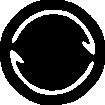
\includegraphics[height=0.4cm, keepaspectratio]{../!config/Bilder/bt_sync_logo.pdf} 
	{\large \textbf{Bittorrent} Sync} \\
	\texttt{B6WH2DISQ5QVYIRYIEZSF4ZR2IDVKPN3I}
	}
\end{minipage}
}


\begin{document}
\pagenumbering{Roman}
\maketitle
\begin{abstract}
\section*{Vorwort --- Mitarbeit am Skript}
Dieses Dokument ist eine Mitschrift aus der Vorlesung \enquote{\fach, \semester}, gelesen von \prof. Der Inhalt entspricht weitestgehend dem Tafelanschrieb. Für die
Korrektheit des Inhalts übernehme ich keinerlei Garantie! Für Bemerkungen und Korrekturen -- und seien es nur Rechtschreibfehler -- bin ich sehr dankbar. 
Korrekturen lassen sich prinzipiell auf drei Wegen einreichen: 
\begin{itemize}
	\item Persönliches Ansprechen in der Uni, Mails an \hrefsymmail{mailto:\mail}{\mail} (gerne auch mit annotieren PDFs) 
	\item \emph{Direktes} Mitarbeiten am Skript: Den Quellcode poste ich auf GitHub (siehe oben), also stehen vielfältige Möglichkeiten der Zusammenarbeit zur Verfügung:
	Zum Beispiel durch Kommentare am Code über die Website und die Kombination Fork + Pull Request. Wer sich verdient macht oder ein Skript zu einer Vorlesung, die 
	ich nicht besuche, beisteuern will, dem gewähre ich gerne auch Schreibzugriff.
	
	Beachten sollte man dabei, dass dazu ein Account bei \url{github.com} notwendig ist, der allerdings ohne Angabe von persönlichen Daten angelegt werden kann. 
	Wer bei GitHub (bzw. dem zugrunde liegenden Open-Source-Programm \enquote{\texttt{git}}) -- verständlicherweise -- Hilfe beim Einstieg braucht, dem helfe ich gerne 
	weiter. Es gibt aber auch zahlreiche empfehlenswerte Tutorials im Internet.\footnote{zB. \url{https://try.github.io/levels/1/challenges/1}, ist auf Englisch, aber dafür 
	interaktives LearningByDoing}
	\item \emph{Indirektes} Mitarbeiten: \TeX-Dateien per Mail verschicken. 
	
	Dies ist nur dann sinnvoll, wenn man einen ganzen Abschnitt ändern möchte (zB. einen alternativen Beweis geben), da ich die Änderungen dann per Hand einbauen muss! Ich freue mich aber auch über solche Beiträge!
\end{itemize}
\section*{Vorlesungshomepage}
{\centering 
\begin{minipage}[c][][c]{\textwidth}
	\centering \qrcode[height=3cm]{\homepage} \medskip\\
	\footnotesize \url{\homepage}
\end{minipage}
\par}

\end{abstract}

\tableofcontents
\cleardoubleoddemptypage

\pagenumbering{arabic}
\setcounter{page}{1}

\section{Kohomologie} % (fold)
\label{sec:1}

\begin{definition}
	Sei $R$ ein Ring. Ein \bet{$R$-Kokettenkomplex}\index{Kokettenkomplex} $(C^*,d^*)$ ist eine Folge von $R$-Moduln $(C^n)_{n \in \mathds{N}}$ zusammen mit $R$-linearen Abbildungen 
	$d^n \colon C^n \to C^{n+1}$, sodass $d^{n+1} \circ d^n =0$. Der \bet{$n$-te Kohomologiemodul}\index{Kohomologiemodul} von $(C^*,d^*)$ ist definiert als 
	\[
		H^n(C^*,d^*) = \frac{\ker d^n \colon C^n \to C^{n+1}}{\im d^{n-1} \colon C^{n-1} \to C^n} 
	\]
	Kokettenabbildungen, Kokettenhomotopien, induzierte Abbildungen, \ldots \todo{hinzufügen}
\end{definition}

\begin{bemerkung} \leavevmode
	\begin{enumerate}[i)]
		\item Sei $(C_*,d_*)$ ein $R$-Kettenkomplex und $V$ ein $R$-Modul. Dann erhalten wir einen $R$"=Kokettenkomplex $(C^*,d^*)$ durch 
		\[
			C^n := \Hom_R(C_n,V) 
		\]
		und $d^n \colon C^n \to C^{n+1}$ definiert durch $\alpha \mapsto \alpha \circ d_{n+1}$. $(C^*,d^*)$ heißt der $V$-duale Kettenkomplex zu $(C_*,d_*)$.
		\item Benutzen wir $\mathds{Z}$ statt $\mathds{N}$ als Indexmenge, so können wir durch $(C^n,d^n) \leadsto (C_n := C^{-n}, d_n := d^{-n})$ jeden Kokettenkomplex einem 
		Kettenkomplex zuordnen. Dieser Prozess ist offensichtlich umkehrbar.
	\end{enumerate}
\end{bemerkung}

\begin{beispiel}
	Sei $(C_*,d_*)= \big(\begin{tikzcd}[cramped] \mathds{Z} & \mathds{Z} \lar["\cdot 2","d_1"'] & 0 \lar & \ldots \lar \end{tikzcd}\big)$ Dann ist
	\[
		H_k(C_*,d_*) = \begin{cases}
			\nicefrac{\mathds{Z}}{2 \mathds{Z}}, &\text{ falls } k =0\\
			0 , & \text{ sonst} 
		\end{cases}
	\]
	Der $\mathds{Z}$-duale Kokettenkomplex ist
	\[
		\begin{tikzcd}
			 \Hom_{\mathds{Z}}(\mathds{Z},\mathds{Z}) \rar["d^1"] \dar["\cong" description] & \Hom_{\mathds{Z}}(\mathds{Z},\mathds{Z}) \rar \dar["\cong" description] 
			& 0 \rar & \ldots \\
			\mathds{Z} \rar["\cdot 2"] & \mathds{Z}
		\end{tikzcd}
	\]
	Damit ist die Kohomologie $H^k(C^*,d^*)$ isomorph zu $\sfrac{\mathds{Z}}{2 \mathds{Z}}$ für $k=1$ und $0$ in jedem anderen Fall.
	Es gilt also nicht immer $H^*(\Hom(C_*;R),d^*) =  \Hom \enbrace{H_*(C_*,d_*),R}$.
\end{beispiel}

\begin{definition}
	Sei $(X,A)$ ein Paar von topologischen Räumen und $V$ eine abelsche Gruppe. Der \Index{singuläre Kokettenkomplex} von $(X,A)$ mit Koeffizienten in $V$ ist definiert durch
	\[
		C^*_\sing(X,A;V) := \Hom_\mathds{Z} \enbrace[\big]{C_*^\sing(X,A),V}
	\]
	und $d^*_\sing(\alpha) := - (-1)^{\abs{\alpha}} \alpha \circ d_*^\sing$. Dabei ist $\abs{\alpha}=n$ für $\alpha \in C^n_\sing(X,A;R)$. Die 
	Kohomologie von $\enbrace*{C^*_\sing(X,A;V), d^*_\sing}$ heißt die \Index{singuläre Kohomologie} von $(X,A)$ mit Koeffizienten in $R$.
\end{definition}

\begin{bemerkung}
	Sei $R$ ein kommutativer Ring und $V$ ein $R$-Modul. Dann ist
	\[
		\enbrace*{C^*_\sing(X,A;V), d^*_\sing}
	\]
	isomorph zum $V$-dualen $R$-Kokettenkomplex des $R$-Kettenkomplexes $\enbrace*{C^\sing_*(X,A;R), d^\sing_*}$.
\end{bemerkung}


\begin{definition}
	Sei $f \colon (X,A) \to (Y,B)$ eine stetige Abbildung von Paaren. Dann erhalten wir eine Kokettenabbildung $f^* \colon C^*_\sing(Y,B;V) \to C^*_\sing(X,A;V)$ durch
	\[
		f^*(\alpha) := \alpha \circ f_*
	\]
\end{definition}

\begin{bemerkung}
	Ist $g \colon (Y,B) \to (Z,C)$ eine weitere Abbildung von Paaren, so gilt $(g \circ f)^* = f^* \circ g^*$.
\end{bemerkung}

\begin{definition}
	Seien $\mathcal{C}$ und $\mathcal{D}$ Kategorien. Ein \Index{kontravarianter Funktor}  $F \colon \mathcal{C} \to \mathcal{D}$ ordnet jedem Objekt $C$ in $\mathcal{C}$ ein Objekt
	$D$ in $\mathcal{D}$ zu und jedem Morphismus $f \colon C \to C'$ einem Morphismus $F(f) \colon F(C') \to F(C)$ in $\mathcal{D}$ zu. Dabei muss gelten:
	\begin{enumerate}[i)]
		\item $F(\id_C)= \id_{F(C)}$
		\item Für $C \xrightarrow{f} C' \xrightarrow{f'}C''$ gilt $F(f' \circ f) = F(f) \circ F(f')$. 
	\end{enumerate}
	Kürzer ist ein \emph{kontravarianter} Funktor $F \colon \mathcal{C} \to \mathcal{D}$ das selbe wie ein \emph{kovarianter} Funktor 
	$\mathcal{C}^\op \to \mathcal{D}^\op$.
\end{definition}

\begin{beispiel}
	\begin{enumerate}[i)]
		\item $\id \colon \mathcal{C} \to \mathcal{C}^\op$ ist kontravariant.
		\item Sei $V$ eine abelsche Gruppe. Wir erhalten einen kontravarianten Funktor
		\[
			\Hom(-,V) \colon \mathds{Z}\text{-}\MOD  \longrightarrow \mathds{Z}\text{-}\MOD
		\]
		\item Sei $V$ eine abelsche Gruppe. Dann sind 
		\begin{align}
			C_\sing^*(-,V) &\colon \TOP^2 \longrightarrow \mathds{Z}\text{-}\textsc{Kokettenkomplexe}  \\
			H^*_\sing \enbrace*{C_\sing^*(_,V),d_\sing^*} &\colon \TOP^2 \longrightarrow \textsc{Gr}\text{-}\mathds{Z}\text{-}\MOD   
		\end{align}
		kontravariante Funktoren.
	\end{enumerate}
\end{beispiel}

\begin{satz}
	Singuläre Kohomologie hat die folgenden Eigenschaften:
	\begin{enumerate}[i)]
		\item \textbf{Dimensionsaxiom:} $H^n_\sing(\set{\pt};V) = V$, falls $n=0$ ist und sonst $0$.\index{Dimensionsaxiom} 
		\item \textbf{Paarfolge:} Es gibt eine natürliche Transformation $\partial^*\colon H^*(A;V) \to H^{*+1}(X,A;V)$ sodass für jedes Paar\index{Paarfolge} 
		\[
			\begin{tikzcd}
				0 \rar & H^0(X,A;V) \rar & H^0(X,V) \rar & H^0(A;V) \rar["\partial"] & H^1(X,A;V) \rar & \ldots 
			\end{tikzcd}
		\]
		eine lange exakte Folge ist. $\partial$ bezeichnet man auch als \Index{verbindende Abbildung}.
		\item \textbf{Ausschneidung:} Sei $L \subseteq A$ mit $\overline{L} \subseteq \mathring{A}$. Dann induziert die Inklusion \index{Ausschneidung}
		$i \colon (X \setminus L, A \setminus L) \hookrightarrow (X,A)$ einen Isomorphismus $i^* \colon H^*(X,A;V) \to H^*(X \setminus L, A \setminus L;V)$.
		\item \textbf{Homotopieinvarianz:} Sind $f,g \colon (X,A) \to (Y,B)$ homotope Abbildungen von Paaren, so gilt $f^* = g^*$ für die induzierten Abbildungen in singulärer 
		Kohomologie.\index{Homotopieinvarianz}
	\end{enumerate}
\end{satz}
\begin{beweis}
	Für singuläre Homologie haben wir die entsprechenden Aussagen schon bewiesen. In allen vier Fällen folgt die Aussage für Kohomologie aus schon bewiesenen Aussagen über 
	den singulären Kettenkomplex.
	
	Wir führen dies an dieser Stelle nur für iv) aus. Seien $f, g \colon X \to Y$ homotop. Dann gibt es eine Kettenhomotopie $H \colon C^\sing_*(X) \to C^\sing_{*+1}(Y)$ zwischen den 
	auf dem singulären Kettenkomplex induzierten Abbildungen $f_*$ und $g_*$. Es gilt also \todo{nochmal durchgucken}
	\[
		d_{n+1} \circ H + H \circ d_n = f_* - g_*
	\]
	$H$ induziert $H^\# \colon C^*_\sing(Y;V) \to C_\sing^*(X;V)$ mit $H^\#(\alpha) := (-1)^{\abs{\alpha}} \alpha \circ H$. Es gilt nun
	\begin{align}
		\enbrace*{d^{n-1} \circ H^\# + H^\# \circ d^n}(\alpha) &= d^{n-1} \circ H^\#(\alpha) + H^\# \circ d^n (\alpha)\\
		&= d^{n-1} \enbrace*{(-1)^n(\alpha \circ H)} - (-1)^n
		H^\# \enbrace*{\alpha \circ d^{n+1}} \\
		&= (-1)^n \enbrace*{(-1)^{n} \alpha \circ H  \circ d_n - (-1)^{n+1} \alpha \circ d_{n+1} \circ H} \\
		&= \alpha \circ H \circ d_n + \alpha \circ d_{n+1} \circ H \\
		&= \alpha \enbrace*{f_* - g_*} = f^*(\alpha) - g^*(\alpha) \qedhere
	\end{align}
\end{beweis}
% section 1 (end)







\cleardoubleoddemptypage
\pagenumbering{Alph}
\setcounter{page}{1}

\printindex
\listoffigures
\todototoc
\listoftodos[To-do's und andere Baustellen]
\end{document}
